% !TEX program = xelatex
\documentclass[12pt,a4paper]{report}

\usepackage{fontspec}
\setmainfont{Times New Roman}
\setsansfont{Arial}
\usepackage{geometry}
\geometry{left=3cm,right=2cm,top=2.5cm,bottom=2.5cm}
\usepackage{graphicx}
\usepackage{booktabs}
\usepackage{longtable}
\usepackage{tabularx}
\usepackage{array}
\usepackage{float}
\usepackage{caption}
\usepackage{subcaption}
\usepackage{amsmath}
\usepackage{enumitem}
\usepackage{setspace}
\usepackage{xcolor}
\usepackage{tikz}
\usepackage{indentfirst}
\usepackage[hidelinks]{hyperref}
\usepackage{bookmark}

\definecolor{sgublue}{RGB}{0,51,102}
\definecolor{lightblue}{RGB}{235,242,250}
\definecolor{lightgray}{RGB}{245,245,245}

\hypersetup{
  colorlinks=true,
  linkcolor=sgublue,
  urlcolor=sgublue,
  citecolor=sgublue
}

\setlength{\parindent}{1cm}
\setlength{\parskip}{4pt}
\setstretch{1.22}
\renewcommand{\arraystretch}{1.25}
\captionsetup{font=small,labelfont=bf}

\renewcommand{\contentsname}{MỤC LỤC}
\renewcommand{\listfigurename}{DANH MỤC HÌNH}
\renewcommand{\listtablename}{DANH MỤC BẢNG}
\renewcommand{\figurename}{Hình}
\renewcommand{\tablename}{Bảng}
\renewcommand{\bibname}{TÀI LIỆU THAM KHẢO}
\renewcommand{\chaptername}{CHƯƠNG}

\begin{document}

% ==================== TRANG BÌA ====================
\begin{titlepage}
\thispagestyle{empty}
\begin{tikzpicture}[remember picture, overlay]
  \draw[line width=1.4pt, color=sgublue]
    ([xshift=1.15cm,yshift=-1.15cm]current page.north west)
    rectangle
    ([xshift=-1.15cm,yshift=1.15cm]current page.south east);
  \draw[line width=0.5pt, color=sgublue]
    ([xshift=1.35cm,yshift=-1.35cm]current page.north west)
    rectangle
    ([xshift=-1.35cm,yshift=1.35cm]current page.south east);
\end{tikzpicture}

\begin{center}
\vspace*{0.15cm}
{\bfseries\large ỦY BAN NHÂN DÂN THÀNH PHỐ HỒ CHÍ MINH}\\[0.12cm]
{\bfseries\Large TRƯỜNG ĐẠI HỌC SÀI GÒN}\\[0.15cm]
{\bfseries\large KHOA TOÁN - ỨNG DỤNG}\\[0.35cm]


\includegraphics[width=3.05cm]{../reports/SGU-LOGO.png}\\[0.35cm]

{\bfseries\Large BÁO CÁO GIỮA KÌ}\\[0.35cm]
{\bfseries\large TÊN ĐỀ TÀI:}\\[0.18cm]
{\bfseries\Large
MULTI-TASK LEARNING CHO PHÂN LOẠI CẢM XÚC\\
VÀ CHỦ ĐỀ PHẢN HỒI SINH VIÊN TIẾNG VIỆT:\\
SO SÁNH TEXTCNN VÀ PHOBERT}\\[0.45cm]

\begin{tabular}{@{}>{\bfseries}p{4.3cm}p{9.0cm}@{}}
Ngành: & Khoa học dữ liệu \\
Môn học: & Lập trình Python nâng cao (858043) \\
Giảng viên hướng dẫn: & TS. Trịnh Tấn Đạt \\
\end{tabular}\\[0.45cm]

{\bfseries\large SINH VIÊN THỰC HIỆN:}\\[0.15cm]
\begin{tabular}{@{}cl@{}}
Đinh Quang Minh & (3123580024) — Nhóm trưởng \\
Dương Tấn Cường & (3123580004) \\
Lê Thành Duy & (3123580007) \\
\end{tabular}
\end{center}

\vfill
\begin{center}
{\bfseries Thành phố Hồ Chí Minh, tháng 11 năm 2026}
\end{center}
\end{titlepage}

% ==================== PHÂN CÔNG ====================
\clearpage
\pagenumbering{roman}
\setcounter{page}{1}
\chapter*{BẢNG PHÂN CÔNG CÔNG VIỆC}
\addcontentsline{toc}{chapter}{BẢNG PHÂN CÔNG CÔNG VIỆC}

Bảng dưới đây trình bày phân công công việc của nhóm. Tỷ lệ đóng góp được chốt theo khối lượng thực hiện:
Đinh Quang Minh 33.4\%, Dương Tấn Cường 33.3\%, Lê Thành Duy 33.3\%.

\begin{table}[H]
\centering
\caption{Bảng phân công công việc của nhóm}
\begin{tabularx}{\textwidth}{@{}c>{\raggedright\arraybackslash}p{3.2cm}c>{\raggedright\arraybackslash}Xc@{}}
\toprule
\textbf{STT} & \textbf{Họ và tên} & \textbf{MSSV} & \textbf{Nội dung công việc chính} & \textbf{Tỷ lệ} \\
\midrule
1 & Đinh Quang Minh & 3123580024 &
Thiết kế pipeline; data loader; EDA; baseline TF-IDF; TextCNN; PhoBERT; keyword-aware; distillation; kiểm định thống kê; demo; tổng hợp báo cáo. &
33.4\% \\
\addlinespace
2 & Dương Tấn Cường & 3123580004 &
Kiểm tra label mapping và data audit; EDA; baseline; TextCNN multi-task; calibration; robustness; review báo cáo và kết quả. &
33.3\% \\
\addlinespace
3 & Lê Thành Duy & 3123580007 &
Tiền xử lý dữ liệu; TextCNN single-task; TextCNN multi-task; student distillation; demo Streamlit; slide/video; kiểm tra tái lập. &
33.3\% \\
\midrule
\multicolumn{4}{@{}r}{\textbf{Tổng cộng}} & \textbf{100.0\%} \\
\bottomrule
\end{tabularx}
\end{table}

\noindent\textit{Ghi chú:} Các đầu việc có tính hỗ trợ chéo; cả ba thành viên cùng tham gia kiểm tra kết quả, đọc báo cáo và chuẩn bị phần bảo vệ.

% ==================== TÓM TẮT ====================
\clearpage
\chapter*{TÓM TẮT}
\addcontentsline{toc}{chapter}{TÓM TẮT}

Phản hồi sinh viên là nguồn dữ liệu quan trọng cho công tác đảm bảo chất lượng giáo dục, nhưng việc đọc và tổng hợp thủ công thường tốn thời gian và dễ bỏ sót vấn đề. Báo cáo này xây dựng một hệ thống multi-task learning để dự đoán đồng thời \textbf{cảm xúc} (tiêu cực, trung tính, tích cực) và \textbf{chủ đề} (giảng viên, chương trình đào tạo, cơ sở vật chất, khác) cho từng câu phản hồi tiếng Việt trên bộ dữ liệu UIT-VSFC.

Nhóm so sánh TextCNN và PhoBERT trong cùng một kiến trúc chia sẻ biểu diễn, sau đó bổ sung \textbf{keyword-aware topic head} với 12 đặc trưng từ khóa và một auxiliary loss. Kết quả trên test cho thấy PhoBERT keyword-aware đạt macro-F1 sentiment 0.7788, macro-F1 topic 0.7633 và joint accuracy 0.8054 ở seed 42. Đánh giá 3 seed cho kết quả trung bình lần lượt 0.7760, 0.7597 và 0.7989, cao hơn PhoBERT frozen ở topic và joint accuracy; kiểm định McNemar và bootstrap xác nhận cải thiện topic/joint nhất quán qua cả 3 seed.

Để triển khai trên CPU, nhóm distill PhoBERT teacher sang TextCNN student. Student chỉ có 407.055 tham số, nhỏ hơn khoảng 332 lần và nhanh hơn khoảng 27.6 lần so với teacher, trong khi vẫn giữ topic-F1 0.7607 và joint accuracy 0.7766 (trung bình 3 seed). Báo cáo cũng đánh giá calibration bằng temperature scaling, robustness với mất dấu/teencode/typo/emoji/đảo trật tự từ, và hạn chế single-label khi câu chứa nhiều chủ đề. Kết quả cho thấy mô hình có giá trị thực tế như một công cụ hỗ trợ phân loại và ưu tiên phản hồi, không thay thế đánh giá của con người.

% ==================== MỤC LỤC ====================
\clearpage
\tableofcontents
\clearpage
\listoffigures
\clearpage
\listoftables

% ==================== CHƯƠNG 1 ====================
\clearpage
\pagenumbering{arabic}
\setcounter{page}{1}
\chapter{GIỚI THIỆU}

\section{Đặt vấn đề}

Trong môi trường đại học, phản hồi của sinh viên là một trong những kênh quan trọng nhất để đánh giá chất lượng giảng dạy, chương trình đào tạo và cơ sở vật chất. Tuy nhiên, dữ liệu này thường tồn tại dưới dạng văn bản tự do, số lượng lớn và không có cấu trúc cố định. Việc đọc thủ công toàn bộ phản hồi vào cuối mỗi học kỳ không chỉ tốn thời gian mà còn khó tổng hợp theo chủ đề và dễ bỏ sót các vấn đề tiêu cực.

Một hệ thống tự động cần trả lời đồng thời hai câu hỏi:

\begin{itemize}[leftmargin=1.2cm]
  \item Phản hồi này thể hiện cảm xúc gì?
  \item Phản hồi này nói về chủ đề nào?
\end{itemize}

Hai câu hỏi có liên quan nhưng không đồng nhất. Một câu có thể tiêu cực về cơ sở vật chất nhưng tích cực về giảng viên; một câu khác có thể trung tính về chương trình đào tạo. Vì vậy, bài toán phù hợp với hướng \textbf{multi-task learning}: dùng chung một biểu diễn đầu vào và tối ưu đồng thời hai đầu ra.

\section{Mục tiêu}

Mục tiêu của đề tài gồm:

\begin{enumerate}[leftmargin=1.2cm]
  \item Xây dựng pipeline tái lập được cho UIT-VSFC: tải dữ liệu, kiểm tra nhãn, tiền xử lý, chia split và đánh giá.
  \item So sánh TextCNN và PhoBERT trong cùng bài toán multi-task tiếng Việt.
  \item Cải thiện topic head bằng đặc trưng từ khóa miền giáo dục và auxiliary loss.
  \item Đánh giá độ ổn định bằng 3 seed, kiểm định thống kê và bootstrap.
  \item Nén mô hình bằng knowledge distillation để chạy trên CPU.
  \item Đánh giá calibration, robustness và xây dựng demo Streamlit có cảnh báo multi-topic.
\end{enumerate}

\section{Phạm vi}

Đề tài tập trung vào phân loại mức câu trên UIT-VSFC, không đi vào aspect-based sentiment hay multi-label. Mô hình PhoBERT được đóng băng để phù hợp điều kiện CPU; không fine-tune toàn bộ encoder. Báo cáo không tuyên bố mô hình thay thế con người trong việc đánh giá giảng viên.

\section{Đóng góp chính}

\begin{itemize}[leftmargin=1.2cm]
  \item Một pipeline multi-task hoàn chỉnh cho UIT-VSFC, có baseline, TextCNN, PhoBERT và kiểm định thống kê.
  \item Một \textbf{keyword-aware PhoBERT} với 12 đặc trưng từ khóa và auxiliary loss, cải thiện topic-F1 và joint accuracy so với PhoBERT frozen.
  \item Một \textbf{TextCNN student} được distill từ PhoBERT, nhỏ hơn 332 lần và nhanh hơn khoảng 27.6 lần trên CPU.
  \item Đánh giá calibration và robustness, chỉ rõ điểm yếu với mất dấu, teencode và câu nhiều chủ đề.
  \item Demo Streamlit có model selector, confidence đã calibration, top-2 chủ đề và cảnh báo multi-topic.
\end{itemize}

\section{Nghiên cứu liên quan}

Bài toán phân tích phản hồi sinh viên nằm ở giao điểm của ba hướng nghiên cứu: phân tích cảm xúc tiếng Việt, multi-task learning và tối ưu mô hình cho triển khai thực tế.

\subsection{Phân tích cảm xúc và chủ đề tiếng Việt}

UIT-VSFC \cite{uitvsfc} là một trong những bộ dữ liệu chuẩn cho phản hồi sinh viên tiếng Việt. Dữ liệu gốc tập trung vào phân loại cảm xúc mức câu; nhãn chủ đề được cung cấp như một bài toán phụ. Các nghiên cứu trước thường dùng TF-IDF, SVM, CNN hoặc BiLSTM. Với sự xuất hiện của PhoBERT \cite{phobert}, các mô hình pretrained nhanh chóng trở thành baseline mạnh cho tiếng Việt nhờ biểu diễn ngữ cảnh tốt hơn.

Tuy nhiên, phần lớn nghiên cứu chỉ tối ưu một task hoặc đánh giá trên một seed. Điều này làm khó so sánh độ ổn định và chưa trả lời rõ câu hỏi: với dữ liệu nhỏ và mất cân bằng, multi-task có thực sự giúp ích không?

\subsection{Multi-task learning}

Caruana \cite{mtl} mô tả multi-task learning như một cách dùng tín hiệu của task phụ để regularize và cải thiện biểu diễn chung. Hai chiến lược phổ biến:

\begin{itemize}[leftmargin=1.2cm]
  \item \textbf{Hard parameter sharing}: dùng chung encoder, tách head ở cuối.
  \item \textbf{Soft parameter sharing}: mỗi task có encoder riêng, ràng buộc tham số giữa các encoder.
\end{itemize}

Đề tài chọn hard sharing vì đơn giản, dễ triển khai trên CPU và phù hợp với hai task có liên quan. Rủi ro chính là \emph{negative transfer}: task này kéo lùi task kia nếu phân bố hoặc độ khó khác nhau. Vì vậy báo cáo không chỉ so sánh multi-task với single-task mà còn kiểm tra per-class và hệ số \(\lambda_t\).

\subsection{TextCNN và transformer}

TextCNN \cite{textcnn} là kiến trúc nhẹ, dùng convolution để bắt n-gram cục bộ. Ưu điểm là tốc độ và khả năng học từ đầu trên dữ liệu nhỏ. Nhược điểm là không mô hình hóa ngữ cảnh xa và phụ thuộc vào chất lượng embedding.

PhoBERT \cite{phobert} khắc phục nhược điểm ngữ cảnh nhưng có chi phí suy luận lớn. Trong điều kiện không GPU, fine-tune toàn bộ PhoBERT là không thực tế; vì vậy đề tài dùng encoder đóng băng và chỉ train head. Đây là điểm cân bằng giữa chất lượng và chi phí.

\subsection{Distillation và triển khai}

Knowledge distillation \cite{distill} chuyển tri thức từ teacher sang student bằng soft label. Hướng này đặc biệt phù hợp khi teacher lớn nhưng môi trường triển khai chỉ có CPU. Thay vì cố gắng fine-tune teacher, đề tài dùng teacher đã có để tạo soft label, sau đó train student TextCNN nhỏ hơn hàng trăm lần.

\subsection{Calibration và robustness}

Các mô hình hiện đại thường quá tự tin; Guo và cộng sự \cite{calibration} chỉ ra rằng confidence không phản ánh đúng xác suất đúng. Temperature scaling là phương pháp hậu xử lý đơn giản, chỉ dùng dev để fit nhiệt độ. Bên cạnh đó, robustness với teencode, mất dấu và lỗi gõ là vấn đề thực tế của dữ liệu mạng xã hội/tiếng Việt.

\subsection{Khoảng trống}

Các công trình riêng lẻ đã giải quyết từng phần: multi-task, PhoBERT, distillation hoặc calibration. Đề tài kết hợp các thành phần này trong một pipeline nhỏ, chạy CPU, có kiểm định thống kê và demo. Đóng góp không nằm ở kiến trúc hoàn toàn mới mà ở việc đánh giá có hệ thống và chuyển hóa kết quả thành công cụ có thể dùng.

\section{Cấu trúc báo cáo}

Chương 2 trình bày dữ liệu và EDA. Chương 3 mô tả phương pháp. Chương 4 trình bày thực nghiệm và kết quả. Chương 5 mô tả demo và ý nghĩa thực tế. Chương 6 trình bày kỹ nghệ phần mềm và tái lập. Chương 7 kết luận và hướng phát triển.


\section*{Tóm tắt chương}
Chương này đặt bài toán, mục tiêu, phạm vi và các đóng góp chính. Điểm cần nhấn mạnh là bài toán không chỉ là phân loại cảm xúc mà còn phải gắn cảm xúc với chủ đề để tạo ra tín hiệu có thể hành động. Chương tiếp theo mô tả dữ liệu và các đặc điểm phân bố ảnh hưởng đến thiết kế mô hình.


% ==================== CHƯƠNG 2 ====================
\chapter{DỮ LIỆU VÀ PHÂN TÍCH KHÁM PHÁ}

\section{Bộ dữ liệu UIT-VSFC}

UIT-VSFC là bộ dữ liệu phản hồi sinh viên tiếng Việt được giới thiệu bởi Nguyen và cộng sự \cite{uitvsfc}. Mỗi mẫu gồm một câu phản hồi, một nhãn cảm xúc và một nhãn chủ đề. Bộ dữ liệu có 16.175 câu, chia thành ba split chính thức.

\begin{table}[H]
\centering
\caption{Quy mô các split của UIT-VSFC}
\begin{tabular}{@{}lrr@{}}
\toprule
\textbf{Split} & \textbf{Số câu} & \textbf{Tỷ lệ} \\
\midrule
Train & 11.426 & 70.6\% \\
Dev & 1.583 & 9.8\% \\
Test & 3.166 & 19.6\% \\
\midrule
Tổng & 16.175 & 100.0\% \\
\bottomrule
\end{tabular}
\end{table}

\section{Nhãn và quy ước}

\begin{table}[H]
\centering
\caption{Mapping nhãn sentiment và topic}
\begin{tabular}{@{}clcl@{}}
\toprule
\textbf{Task} & \textbf{ID} & \textbf{Nhãn} & \textbf{Ý nghĩa} \\
\midrule
Sentiment & 0 & negative & Tiêu cực \\
Sentiment & 1 & neutral & Trung tính \\
Sentiment & 2 & positive & Tích cực \\
\midrule
Topic & 0 & lecturer & Giảng viên \\
Topic & 1 & training\_program & Chương trình đào tạo \\
Topic & 2 & facility & Cơ sở vật chất \\
Topic & 3 & others & Khác \\
\bottomrule
\end{tabular}
\end{table}

Thứ tự nhãn được đọc từ \texttt{configs/label\_map.json} và kiểm tra bằng ví dụ thực tế, không hardcode theo cảm tính.

\section{Phân bố nhãn}

\begin{table}[H]
\centering
\caption{Phân bố nhãn sentiment theo split}
\begin{tabular}{@{}lrrr@{}}
\toprule
\textbf{Split} & \textbf{negative} & \textbf{neutral} & \textbf{positive} \\
\midrule
Train & 5.325 & 458 & 5.643 \\
Dev & 705 & 73 & 805 \\
Test & 1.409 & 167 & 1.590 \\
\bottomrule
\end{tabular}
\end{table}

\begin{table}[H]
\centering
\caption{Phân bố nhãn topic theo split}
\begin{tabular}{@{}lrrrr@{}}
\toprule
\textbf{Split} & \textbf{lecturer} & \textbf{training\_program} & \textbf{facility} & \textbf{others} \\
\midrule
Train & 8.166 & 2.201 & 497 & 562 \\
Dev & 1.151 & 267 & 70 & 95 \\
Test & 2.290 & 572 & 145 & 159 \\
\bottomrule
\end{tabular}
\end{table}

Hai đặc điểm mất cân bằng nổi bật:

\begin{itemize}[leftmargin=1.2cm]
  \item \texttt{neutral} chỉ chiếm khoảng 4.0\% train, nên accuracy dễ gây ấn tượng sai; báo cáo dùng macro-F1.
  \item \texttt{lecturer} chiếm khoảng 71.5\% train; các lớp \texttt{facility} và \texttt{others} ít hơn nhiều.
\end{itemize}

\begin{figure}[H]
\centering
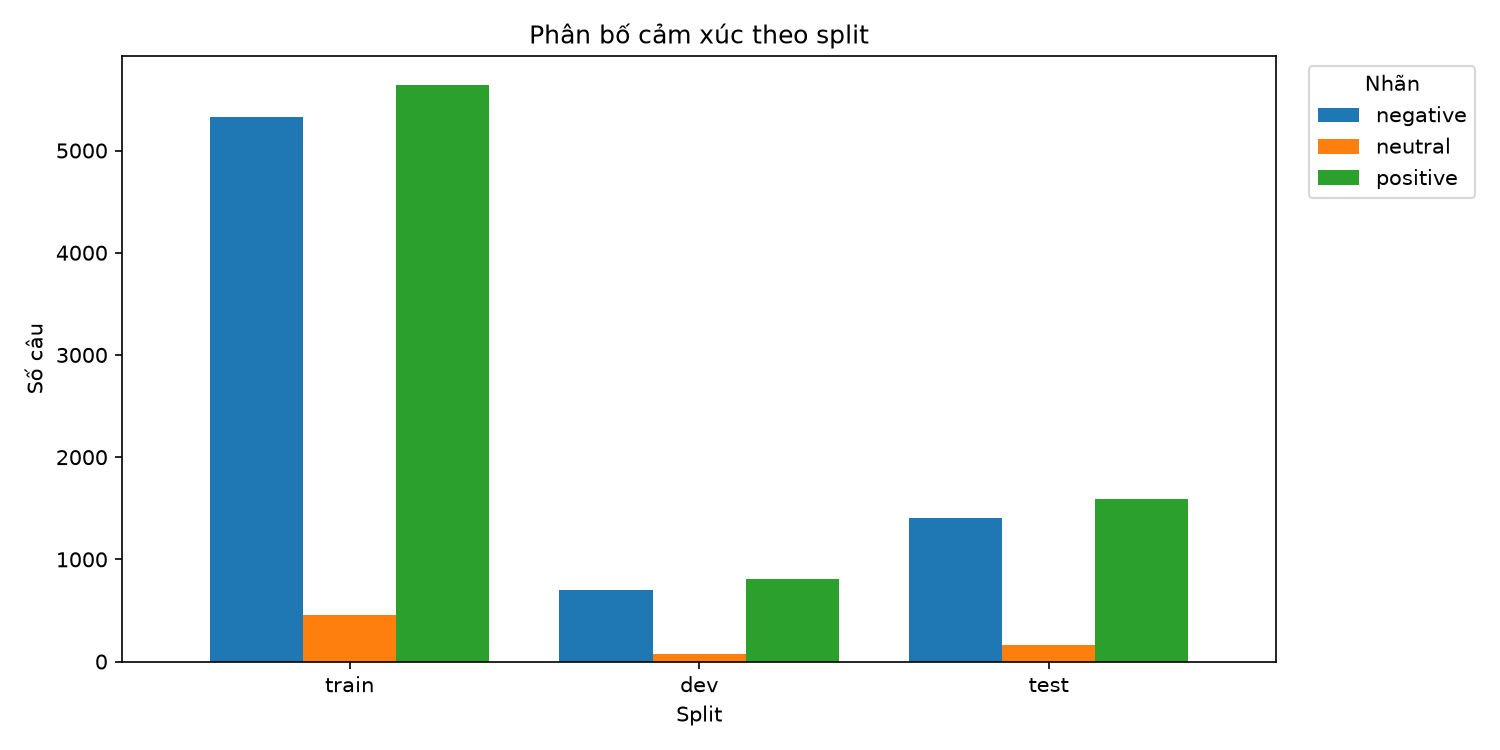
\includegraphics[width=0.60\textwidth]{../reports/data/figures/sentiment_distribution.png}
\caption{Phân bố cảm xúc trong tập train}
\end{figure}

\begin{figure}[H]
\centering
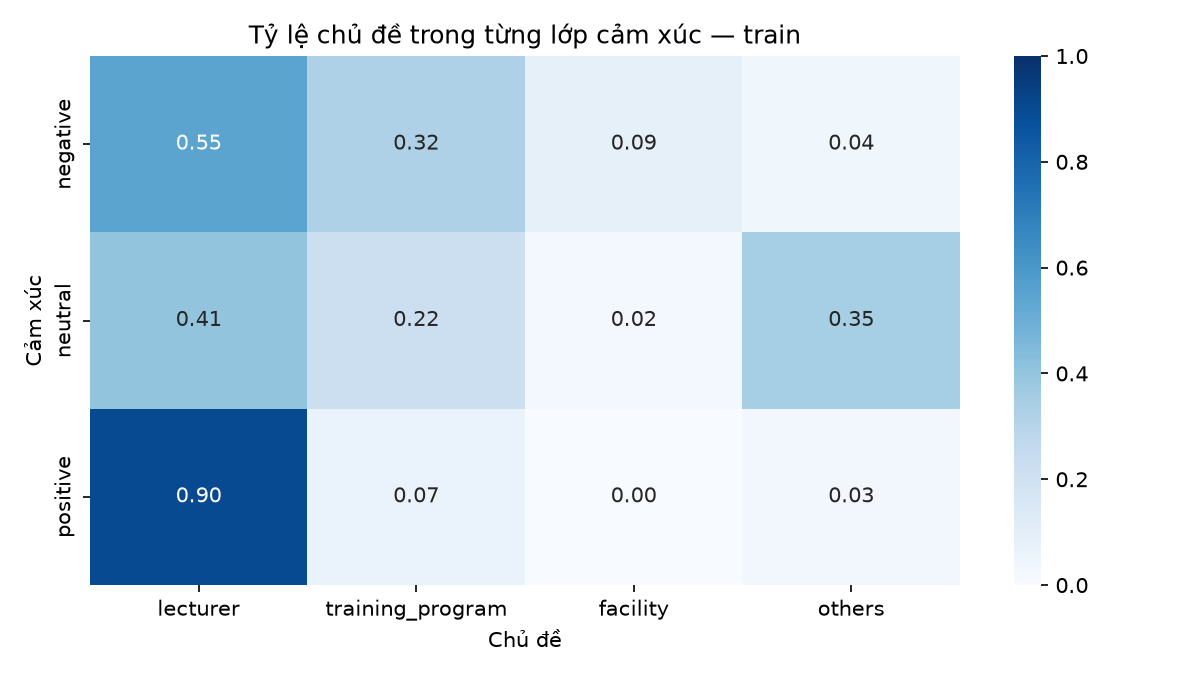
\includegraphics[width=0.58\textwidth]{../reports/data/figures/sentiment_topic_heatmap.png}
\caption{Tương quan giữa cảm xúc và chủ đề}
\end{figure}

\section{Nhận xét EDA}

Các phát hiện chính:

\begin{itemize}[leftmargin=1.2cm]
  \item p95 độ dài câu train là 33 token; chọn \texttt{max\_len=48} để cân bằng độ phủ và chi phí.
  \item Không có câu rỗng; không có trùng lặp giữa train/dev/test.
  \item Trong train có 1 câu trùng nội bộ; chưa xử lý nhưng ghi nhận.
  \item \texttt{facility} gần như luôn tiêu cực: 474/497 câu train.
  \item Sentiment và topic có tương quan mạnh, tạo nguy cơ shortcut: model có thể học “cứ facility là negative” thay vì học ngữ nghĩa.
\end{itemize}

Những đặc điểm này định hướng thiết kế: dùng class weight, macro-F1, kiểm tra per-class và phân tích lỗi định tính.


\section*{Tóm tắt chương}
Chương này mô tả nguồn dữ liệu, quy ước nhãn và các đặc điểm mất cân bằng. Các phát hiện EDA giải thích vì sao báo cáo dùng macro-F1, class weight và phân tích per-class thay vì chỉ báo cáo accuracy. Chương tiếp theo trình bày kiến trúc TextCNN, PhoBERT, keyword-aware head và distillation.


% ==================== CHƯƠNG 3 ====================
\chapter{PHƯƠNG PHÁP}

\section{Phát biểu bài toán}

Cho câu phản hồi \(x\) được tách thành chuỗi token \(x = (x_1, \ldots, x_n)\). Ta cần dự đoán:

\[
y_s \in \{\text{negative}, \text{neutral}, \text{positive}\}, \qquad
y_t \in \{\text{lecturer}, \text{training\_program}, \text{facility}, \text{others}\}.
\]

Với multi-task hard parameter sharing, model có một encoder chung và hai head. Hàm mất mát:

\begin{equation}
\mathcal{L} = \mathcal{L}_s + \lambda_t \mathcal{L}_t,
\end{equation}

trong đó \(\mathcal{L}_s\) và \(\mathcal{L}_t\) là cross-entropy cho sentiment và topic; \(\lambda_t\) điều chỉnh mức ảnh hưởng của topic.

\section{Tiền xử lý}

Quy trình tiền xử lý:

\begin{enumerate}[leftmargin=1.2cm]
  \item Chuẩn hóa Unicode NFC và khoảng trắng.
  \item Tách từ tiếng Việt bằng \texttt{underthesea}.
  \item Xây vocabulary chỉ trên train, min frequency 2, tối đa 50.000 token.
  \item Encode/Pad về \texttt{max\_len=48}.
  \item Với PhoBERT, dùng tokenizer chính thức của \texttt{vinai/phobert-base}.
\end{enumerate}

Việc chỉ fit vocabulary trên train nhằm tránh rò rỉ dữ liệu.

\section{TextCNN}

TextCNN \cite{textcnn} dùng các convolution một chiều với kernel 3, 4, 5 để bắt n-gram cục bộ:

\begin{itemize}[leftmargin=1.2cm]
  \item Embedding 100 chiều.
  \item 100 filter cho mỗi kernel.
  \item Max-pooling theo thời gian.
  \item Shared hidden 256, dropout 0.5.
  \item Hai head tuyến tính cho sentiment và topic.
\end{itemize}

Mô hình có khoảng 0.41 triệu tham số, phù hợp CPU.

\section{PhoBERT frozen}

PhoBERT \cite{phobert} là encoder tiếng Việt dựa trên RoBERTa. Trong đề tài, encoder được đóng băng; embedding \texttt{[CLS]} 768 chiều được trích một lần và cache:

\[
\mathbf{h} = \text{PhoBERT}(x)_{[\text{CLS}]}.
\]

Sau đó:

\[
\mathbf{z} = \mathrm{Dropout}(\mathrm{ReLU}(\mathbf{W}\mathbf{h} + \mathbf{b})),
\]

và hai head dự đoán sentiment/topic. Cách này giữ chi phí huấn luyện thấp trên CPU nhưng vẫn tận dụng biểu diễn ngữ nghĩa mạnh của PhoBERT.

\section{Keyword-aware topic head}

Phân tích lỗi cho thấy các cụm như \texttt{giảng\_viên}, \texttt{cơ\_sở}, \texttt{vật\_chất}, \texttt{chương\_trình} là tín hiệu miền rất mạnh. Nhóm bổ sung 12 đặc trưng:

\begin{itemize}[leftmargin=1.2cm]
  \item Với mỗi trong 4 topic: có keyword xuất hiện không.
  \item Mật độ keyword trong câu.
  \item Keyword có nằm trong 3 token cuối không.
\end{itemize}

Topic head nhận concatenation của shared hidden và vector keyword:

\[
\mathbf{u} = [\mathbf{z}; \mathbf{k}], \qquad
\boldsymbol{\ell}_t = \mathbf{W}_t \mathbf{u} + \mathbf{b}_t + \alpha \mathbf{W}_k \mathbf{k}.
\]

Thêm một auxiliary loss buộc keyword head học trực tiếp từ keyword:

\begin{equation}
\mathcal{L} = \mathcal{L}_s + \lambda_t \mathcal{L}_t + \beta \mathcal{L}_{kw},
\end{equation}

với \(\beta=0.5\). Nhóm cũng dùng \texttt{sqrt\_balanced} class weight để giảm thiên vị về lớp đa số.

\section{Knowledge distillation}

Teacher là PhoBERT keyword-aware; student là TextCNN multi-task. Soft label của teacher được cache cho train/dev/test. Student tối ưu:

\begin{equation}
\mathcal{L} = \mathcal{L}_{hard} + \beta T^2
\mathrm{KL}\left(\mathrm{softmax}(\mathbf{z}^{teacher}/T) \,\|\, \mathrm{softmax}(\mathbf{z}^{student}/T)\right),
\end{equation}

với \(T=2.0\), \(\beta=0.5\), \(\lambda_t=1.0\). Mục tiêu không phải vượt teacher mà là giữ chất lượng gần teacher với chi phí nhỏ hơn nhiều.

\section{Giao thức huấn luyện}

\begin{itemize}[leftmargin=1.2cm]
  \item Chọn model bằng dev mean macro-F1; test chỉ đánh giá một lần cho cấu hình cuối.
  \item Early stopping theo dev; seed 42, 123, 2024 cho đánh giá 3 seed.
  \item TextCNN: Adam, learning rate \(10^{-3}\), batch 32, tối đa 20 epoch.
  \item PhoBERT head: Adam, learning rate \(10^{-3}\), batch 32, tối đa 30 epoch.
  \item Không fine-tune encoder PhoBERT.
\end{itemize}

\section{Thiết kế thực nghiệm}

Thực nghiệm được chia thành các giai đoạn độc lập để dễ truy vết và tránh tune trên test.

\begin{table}[H]
\centering
\caption{Ma trận thực nghiệm}
\begin{tabularx}{\textwidth}{@{}clXc@{}}
\toprule
\textbf{ID} & \textbf{Mô hình} & \textbf{Mục đích} & \textbf{Seed} \\
\midrule
E0 & Data audit + EDA & Kiểm tra nhãn, phân bố, trùng lặp, độ dài & -- \\
E1 & TF-IDF + Logistic Regression & Baseline tuyến tính, dễ giải thích & 42 \\
E2 & TextCNN single-task & Baseline học sâu nhẹ, train từ đầu & 42 \\
E3 & TextCNN multi-task & Đo ảnh hưởng của chia sẻ tham số & 42, 123, 2024 \\
E4 & PhoBERT frozen multi-task & Tận dụng pretrained encoder trên CPU & 42, 123, 2024 \\
E5 & PhoBERT keyword-aware & Đo ảnh hưởng của keyword + auxiliary loss & 42, 123, 2024 \\
E6 & TextCNN distilled & Nén teacher thành student nhỏ & 42, 123, 2024 \\
E7 & Calibration + robustness & Đánh giá độ tin cậy và độ bền & 42 \\
\bottomrule
\end{tabularx}
\end{table}

Các biến kiểm soát:

\begin{itemize}[leftmargin=1.2cm]
  \item Cùng split chính thức; không trộn test vào train.
  \item Cùng metric: macro-F1 và joint accuracy.
  \item Model selection chỉ dùng dev mean-F1.
  \item Với TextCNN, giữ nguyên kiến trúc khi so single/multi.
  \item Với PhoBERT, giữ nguyên encoder frozen khi so frozen/keyword.
  \item Mỗi cấu hình cuối được đánh giá test một lần; kết quả 3 seed báo cáo mean \(\pm\) std.
\end{itemize}

Một số ablation không chạy đầy đủ do giới hạn thời gian, ví dụ grid search toàn bộ \(\lambda_t\), temperature, hoặc số layer fine-tune. Báo cáo chỉ kết luận từ các cấu hình đã chạy và ghi rõ phần chưa kiểm chứng.

\section{Độ đo và kiểm định}

\begin{itemize}[leftmargin=1.2cm]
  \item \textbf{Macro-F1} cho từng task, phù hợp mất cân bằng lớp.
  \item \textbf{Joint accuracy}: tỷ lệ câu đúng cả sentiment và topic.
  \item \textbf{McNemar exact test} trên correctness từng câu.
  \item \textbf{Bootstrap 95\% CI} cho chênh lệch macro-F1/accuracy.
  \item \textbf{ECE} (Expected Calibration Error) cho calibration.
  \item \textbf{Robustness}: mất dấu, teencode, typo, emoji, đảo trật tự từ.
\end{itemize}


\section*{Tóm tắt chương}
Chương này trình bày công thức multi-task, cách tiền xử lý, kiến trúc TextCNN, PhoBERT frozen, keyword-aware head và knowledge distillation. Giao thức huấn luyện được thiết kế để chọn model bằng dev, đánh giá test một lần và lặp lại với 3 seed. Chương tiếp theo trình bày kết quả thực nghiệm và các kiểm định.


% ==================== CHƯƠNG 4 ====================
\chapter{THỰC NGHIỆM VÀ KẾT QUẢ}

\section{Môi trường thực nghiệm}

\begin{table}[H]
\centering
\caption{Cấu hình thực nghiệm}
\begin{tabular}{@{}ll@{}}
\toprule
\textbf{Thành phần} & \textbf{Giá trị} \\
\midrule
Python & 3.12.15 \\
PyTorch & 2.14.1+cpu \\
Transformers & 5.20.2 \\
Device & CPU \\
Encoder & \texttt{vinai/phobert-base} (frozen) \\
TextCNN & embedding 100, filters 100, kernel 3/4/5 \\
Seeds & 42, 123, 2024 \\
\bottomrule
\end{tabular}
\end{table}

\section{Kết quả một seed}

\begin{table}[H]
\centering
\caption{Kết quả test seed 42}
\begin{tabular}{@{}lrrr@{}}
\toprule
\textbf{Model} & \textbf{Sentiment F1} & \textbf{Topic F1} & \textbf{Joint} \\
\midrule
TF-IDF + Logistic Regression & 0.7400 & 0.7247 & 0.7227 \\
TextCNN single-task & 0.7621 & 0.7355 & 0.7536 \\
TextCNN multi-task & 0.7556 & 0.7390 & 0.7552 \\
PhoBERT frozen multi-task & 0.7785 & 0.7428 & 0.7855 \\
\textbf{PhoBERT keyword-aware} & \textbf{0.7788} & \textbf{0.7633} & \textbf{0.8054} \\
\bottomrule
\end{tabular}
\end{table}

Nhận xét:

\begin{itemize}[leftmargin=1.2cm]
  \item TextCNN multi-task chưa cải thiện rõ so với single-task; có dấu hiệu negative transfer nhẹ ở sentiment.
  \item PhoBERT frozen tăng mạnh sentiment và joint so với TextCNN.
  \item Keyword-aware gần như giữ nguyên sentiment nhưng tăng topic 0.0205 và joint 0.0199 so với PhoBERT frozen.
\end{itemize}

\section{Kết quả 3 seed}

\begin{table}[H]
\centering
\caption{Test mean \(\pm\) std trên 3 seed}
\begin{tabular}{@{}lccc@{}}
\toprule
\textbf{Model} & \textbf{Sentiment F1} & \textbf{Topic F1} & \textbf{Joint} \\
\midrule
TextCNN multi-task & 0.7559 \(\pm\) 0.0024 & 0.7508 \(\pm\) 0.0103 & 0.7654 \(\pm\) 0.0090 \\
PhoBERT frozen & 0.7679 \(\pm\) 0.0101 & 0.7388 \(\pm\) 0.0082 & 0.7612 \(\pm\) 0.0291 \\
\textbf{PhoBERT keyword-aware} & \textbf{0.7760 \(\pm\) 0.0060} & \textbf{0.7597 \(\pm\) 0.0067} & \textbf{0.7989 \(\pm\) 0.0059} \\
\bottomrule
\end{tabular}
\end{table}

Keyword-aware có mean tốt nhất ở cả ba metric và phương sai joint thấp hơn nhiều so với PhoBERT frozen. Điều này cho thấy cải thiện không chỉ đến từ một seed may mắn.

\section{Kiểm định thống kê}

\begin{table}[H]
\centering
\caption{Tóm tắt McNemar và bootstrap trên 3 seed}
\begin{tabular}{@{}llcc@{}}
\toprule
\textbf{So sánh} & \textbf{Task} & \textbf{McNemar p<0.05} & \textbf{CI loại 0} \\
\midrule
keyword vs frozen & topic & 3/3 & 3/3 \\
keyword vs frozen & joint & 3/3 & 3/3 \\
keyword vs frozen & sentiment & 3/3 & 1/3 \\
keyword vs TextCNN & joint & 3/3 & 3/3 \\
keyword vs TextCNN & topic & 1/3 & 1/3 \\
keyword vs TextCNN & sentiment & 3/3 & 0/3 \\
\bottomrule
\end{tabular}
\end{table}

Kết luận thống kê:

\begin{itemize}[leftmargin=1.2cm]
  \item Cải thiện \textbf{topic} so với PhoBERT frozen là nhất quán.
  \item Cải thiện \textbf{joint accuracy} so với cả PhoBERT frozen và TextCNN là nhất quán.
  \item Chưa đủ bằng chứng để khẳng định cải thiện sentiment F1.
  \item So với TextCNN, lợi thế topic không ổn định qua các seed.
\end{itemize}

\section{Ablation và phân tích per-class}

Bảng \ref{tab:ablation} tổng hợp các so sánh có kiểm soát. Mỗi cặp chỉ thay một thành phần để có thể quy kết phần nào tạo ra chênh lệch.

\begin{table}[H]
\centering
\caption{Ablation từ các cấu hình có sẵn (test, seed 42)}
\label{tab:ablation}
\begin{tabularx}{\textwidth}{@{}lXrrr@{}}
\toprule
\textbf{So sánh} & \textbf{Thay đổi} & \textbf{\(\Delta\) Sent} & \textbf{\(\Delta\) Topic} & \textbf{\(\Delta\) Joint} \\
\midrule
TextCNN single \(\rightarrow\) multi & Chia sẻ encoder, thêm topic head & -0.0065 & +0.0035 & +0.0016 \\
PhoBERT frozen \(\rightarrow\) keyword & Thêm 12 keyword + aux loss & +0.0003 & +0.0205 & +0.0199 \\
TextCNN hard \(\rightarrow\) distilled & Học thêm soft label của teacher & +0.0068 & +0.0099 & +0.0112 \\
\bottomrule
\end{tabularx}
\end{table}

Diễn giải:

\begin{itemize}[leftmargin=1.2cm]
  \item Multi-task TextCNN \textbf{không} cải thiện sentiment; có dấu hiệu negative transfer nhẹ. Topic tăng nhẹ nhưng chưa đủ lớn để kết luận.
  \item Keyword features cải thiện topic rõ rệt nhưng gần như không đổi sentiment, đúng với thiết kế chỉ can thiệp vào topic head.
  \item Distillation cải thiện cả ba metric so với student hard-label, cho thấy soft label của teacher có tác dụng regularize.
\end{itemize}

\begin{table}[H]
\centering
\caption{Per-class test của PhoBERT keyword-aware (seed 42)}
\begin{tabular}{@{}llrrr@{}}
\toprule
\textbf{Task} & \textbf{Lớp} & \textbf{Precision} & \textbf{Recall} & \textbf{F1} \\
\midrule
Sentiment & negative & 0.9262 & 0.9446 & 0.9353 \\
Sentiment & neutral & 0.4966 & 0.4311 & 0.4615 \\
Sentiment & positive & 0.9413 & 0.9377 & 0.9395 \\
\midrule
Topic & lecturer & 0.9235 & 0.9284 & 0.9260 \\
Topic & training\_program & 0.7518 & 0.7255 & 0.7384 \\
Topic & facility & 0.8766 & 0.9310 & 0.9030 \\
Topic & others & 0.4873 & 0.4843 & 0.4858 \\
\bottomrule
\end{tabular}
\end{table}

Hai điểm đáng chú ý:

\begin{itemize}[leftmargin=1.2cm]
  \item \texttt{neutral} vẫn là lớp khó nhất (F1 0.4615), do chỉ có 167 mẫu test và tín hiệu từ vựng mờ.
  \item \texttt{others} có F1 thấp (0.4858), vì đây là lớp “phần còn lại”, không có keyword đặc trưng và rất đa dạng.
\end{itemize}

\section{Phân tích lỗi}

Một lỗi tiêu biểu là câu:

\begin{quote}
\textit{“cần phải cải thiện thêm, nhất là giảng viên”}
\end{quote}

PhoBERT frozen dự đoán facility 99.0\%. Sau khi thêm keyword features và auxiliary loss, model dự đoán lecturer 49.9\% (facility 44.5\%) — đúng nhãn nhưng confidence thấp. Đây là hành vi hợp lý hơn so với việc tự tin sai.

Một lỗi khác là câu nhiều chủ đề:

\begin{quote}
\textit{“giảng viên tệ, cơ sở vật chất lỏ”}
\end{quote}

Model dự đoán facility 83.7\%, lecturer 15.6\%. Đây không phải lỗi softmax: bài toán hiện là single-label, nên model chỉ chọn chủ đề trội. Demo đã thêm cảnh báo multi-topic và hiển thị top-2 để tránh hiểu nhầm.

\section{Knowledge distillation}

\begin{table}[H]
\centering
\caption{So sánh teacher, hard-label student và distilled student (3 seed)}
\begin{tabular}{@{}lccc@{}}
\toprule
\textbf{Model} & \textbf{Sentiment F1} & \textbf{Topic F1} & \textbf{Joint} \\
\midrule
PhoBERT teacher & \textbf{0.7760 \(\pm\) 0.0060} & 0.7597 \(\pm\) 0.0067 & \textbf{0.7989 \(\pm\) 0.0059} \\
TextCNN hard-label & 0.7559 \(\pm\) 0.0024 & 0.7508 \(\pm\) 0.0103 & 0.7654 \(\pm\) 0.0090 \\
\textbf{TextCNN distilled} & 0.7627 \(\pm\) 0.0047 & \textbf{0.7607 \(\pm\) 0.0102} & 0.7766 \(\pm\) 0.0087 \\
\bottomrule
\end{tabular}
\end{table}

\begin{table}[H]
\centering
\caption{Chi phí suy luận trên CPU (100 câu test)}
\begin{tabular}{@{}lrrr@{}}
\toprule
\textbf{Metric} & \textbf{Teacher} & \textbf{Student} & \textbf{Tỷ lệ} \\
\midrule
Parameters & 135.198.571 & 407.055 & 332\(\times\) ít hơn \\
Estimated size & 515.74 MB & 1.55 MB & 332\(\times\) nhỏ hơn \\
Latency & 63.68 ms/câu & 2.30 ms/câu & 27.6\(\times\) nhanh hơn \\
Throughput & 15.7 câu/s & 433.9 câu/s & 27.6\(\times\) \\
\bottomrule
\end{tabular}
\end{table}

Distillation tăng đều cả ba metric so với TextCNN hard-label. Student gần như ngang teacher ở topic, thấp hơn ở sentiment/joint, nhưng nhỏ và nhanh hơn rất nhiều. Đây là trade-off phù hợp cho triển khai CPU.

\section{Calibration}

\begin{table}[H]
\centering
\caption{ECE trước và sau temperature scaling trên test}
\begin{tabular}{@{}llrrr@{}}
\toprule
\textbf{Model} & \textbf{Task} & \textbf{T} & \textbf{ECE trước} & \textbf{ECE sau} \\
\midrule
Teacher & sentiment & 1.366 & 0.0242 & 0.0215 \\
Teacher & topic & 1.230 & 0.0254 & \textbf{0.0097} \\
Student & sentiment & 1.930 & 0.0658 & \textbf{0.0166} \\
Student & topic & 1.823 & 0.0805 & \textbf{0.0145} \\
\bottomrule
\end{tabular}
\end{table}

Student overconfident hơn teacher trước calibration. Sau temperature scaling, ECE giảm mạnh, đặc biệt ở student. Accuracy không đổi vì temperature chỉ sửa confidence, không sửa argmax.

\begin{figure}[H]
\centering
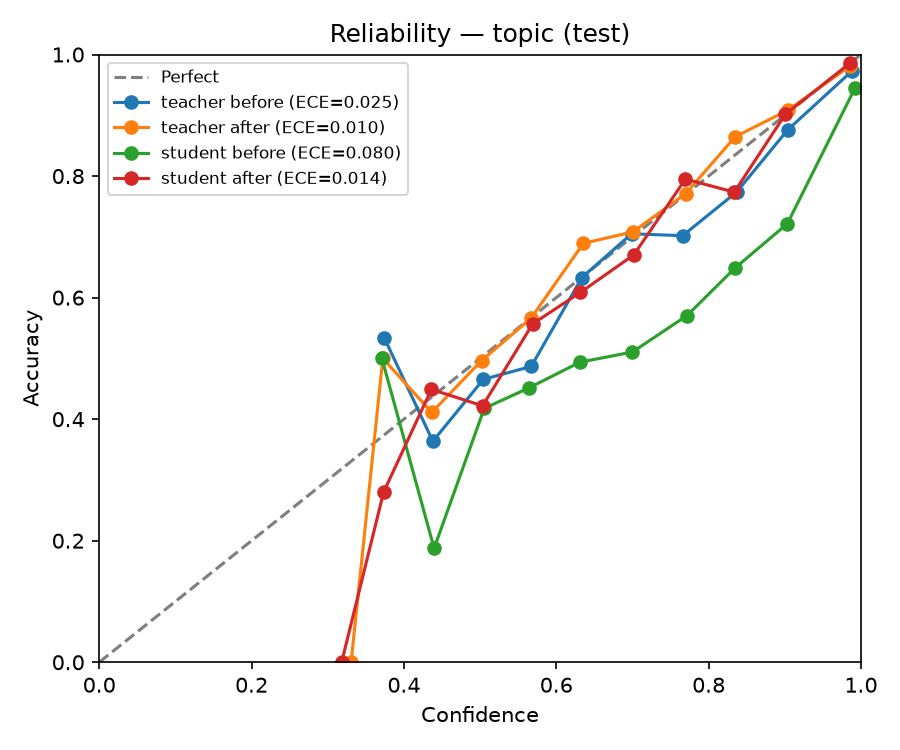
\includegraphics[width=0.72\textwidth]{../reports/evaluation/figures/calibration_topic_reliability.png}
\caption{Reliability diagram cho topic sau calibration}
\end{figure}

\section{Robustness}

\begin{table}[H]
\centering
\caption{Topic-F1 dưới các perturbation (800 câu test)}
\begin{tabular}{@{}lrr@{}}
\toprule
\textbf{Variant} & \textbf{Teacher} & \textbf{Student} \\
\midrule
Clean & 0.7727 & 0.7322 \\
Không dấu & 0.1517 & 0.1165 \\
Teencode & 0.6833 & 0.6303 \\
Typo & 0.7699 & 0.7005 \\
Emoji & 0.6661 & \textbf{0.7440} \\
Đảo trật tự từ & 0.6678 & \textbf{0.7099} \\
\bottomrule
\end{tabular}
\end{table}

\begin{figure}[H]
\centering
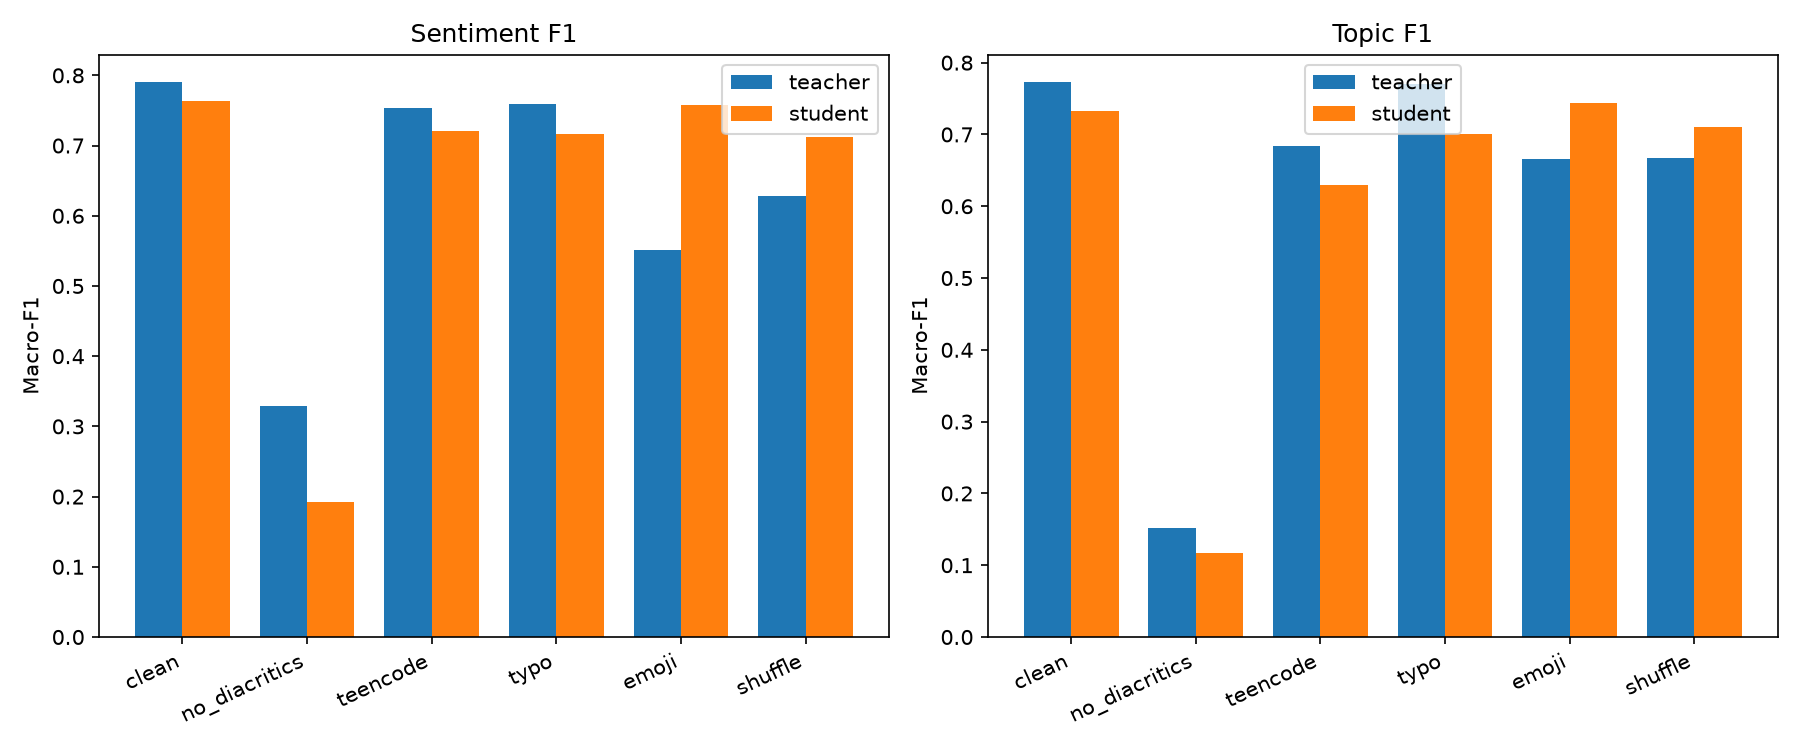
\includegraphics[width=0.82\textwidth]{../reports/evaluation/figures/robustness_scores.png}
\caption{So sánh robustness của teacher và student}
\end{figure}

Kết quả cho thấy mất dấu là điểm yếu nghiêm trọng nhất của cả hai mô hình. Teacher nhạy với emoji và đảo trật tự từ hơn student; student bền vững hơn ở hai perturbation này nhưng yếu hơn ở clean test.


\section*{Tóm tắt chương}
Chương này trình bày kết quả một seed, kết quả 3 seed, kiểm định McNemar/bootstrap, ablation, per-class, distillation, calibration và robustness. Kết quả cho thấy keyword-aware PhoBERT cải thiện topic/joint, còn student distilled là trade-off hợp lý cho CPU. Chương tiếp theo mô tả demo và ý nghĩa thực tế.


% ==================== CHƯƠNG 5 ====================
\section{Thảo luận}

\subsection{TextCNN và PhoBERT}

Kết quả cho thấy PhoBERT frozen vượt TextCNN ở sentiment và joint, nhưng khoảng cách topic không lớn. Điều này hợp lý vì:

\begin{itemize}[leftmargin=1.2cm]
  \item PhoBERT đã học ngữ cảnh tiếng Việt từ corpus lớn, trong khi TextCNN chỉ học từ 11.426 câu train.
  \item Topic phụ thuộc mạnh vào keyword bề mặt; TextCNN với convolution 3/4/5 đã bắt được các cụm này khá tốt.
  \item Sentiment cần hiểu phủ định, mức độ và ngữ cảnh, nơi PhoBERT có lợi thế rõ hơn.
\end{itemize}

\subsection{TextCNN multi-task có thực sự tốt hơn?}

Không có bằng chứng nhất quán. Sentiment giảm nhẹ, topic tăng nhẹ, joint gần như không đổi. Có hai cách giải thích:

\begin{itemize}[leftmargin=1.2cm]
  \item Hai task có tương quan nhưng không hoàn toàn đồng nhất; hard sharing có thể gây negative transfer.
  \item TextCNN nhỏ, dung lượng hạn chế; chia sẻ hidden 256 cho hai head có thể tạo nút thắt.
\end{itemize}

Vì vậy báo cáo không tuyên bố multi-task luôn tốt hơn. Kết luận đúng là: với cấu hình này, multi-task không cải thiện rõ TextCNN, nhưng là nền tảng để thêm keyword head và distillation.

\subsection{Keyword-aware: lợi ích và rủi ro}

Keyword features giúp topic tăng 0.0205 so với PhoBERT frozen. Đây là mức cải thiện có ý nghĩa thống kê qua 3 seed. Tuy nhiên, cách làm này có rủi ro:

\begin{itemize}[leftmargin=1.2cm]
  \item Nếu keyword xuất hiện nhưng không phải chủ đề chính, model có thể bị kéo sai.
  \item Keyword list do con người thiết kế, có thể thiên lệch theo tập train.
  \item Câu không chứa keyword vẫn phụ thuộc hoàn toàn vào encoder.
\end{itemize}

Trong báo cáo, keyword được xem là \emph{inductive bias} có kiểm soát, không phải rule cứng.

\subsection{Teacher hay student?}

Hai mô hình phục vụ hai mục đích khác nhau:

\begin{itemize}[leftmargin=1.2cm]
  \item \textbf{Teacher}: dùng khi cần chất lượng cao nhất, chấp nhận 63.68 ms/câu.
  \item \textbf{Student}: dùng khi cần throughput, chạy CPU, hoặc triển khai nội bộ với chi phí thấp.
\end{itemize}

Student nhỏ hơn 332 lần nhưng chỉ giảm khoảng 0.022 joint accuracy so với teacher. Đây là trade-off hợp lý cho nhiều kịch bản thực tế.

\subsection{Câu nhiều chủ đề}

Bài toán hiện là single-label. Với câu như “giảng viên tệ, cơ sở vật chất lỏ”, model buộc phải chọn một chủ đề. Demo đã cảnh báo và hiển thị top-2, nhưng về bản chất đây là giới hạn của dữ liệu, không phải lỗi softmax. Muốn giải quyết đúng cần multi-label annotation.

\subsection{Threats to validity}

\begin{itemize}[leftmargin=1.2cm]
  \item \textbf{Internal validity}: cùng một pipeline, cùng split; đã kiểm tra trùng lặp. Tuy nhiên chưa chạy full grid hyperparameter.
  \item \textbf{External validity}: chỉ đánh giá trên UIT-VSFC, chưa cross-domain.
  \item \textbf{Construct validity}: topic là nhãn mức câu, không phải aspect; sentiment cũng mức câu.
  \item \textbf{Statistical validity}: 3 seed là nhỏ; McNemar/bootstrap giúp nhưng không thay thế nhiều seed hơn.
\end{itemize}

\chapter{DEMO VÀ Ý NGHĨA THỰC TẾ}

\section{Kiến trúc demo}

Demo được xây dựng bằng Streamlit, cho phép chọn:

\begin{itemize}[leftmargin=1.2cm]
  \item \textbf{PhoBERT teacher}: chính xác hơn, chậm hơn.
  \item \textbf{TextCNN student}: nhỏ, nhanh, phù hợp CPU.
\end{itemize}

Mỗi dự đoán hiển thị:

\begin{itemize}[leftmargin=1.2cm]
  \item nhãn cảm xúc và chủ đề;
  \item confidence đã calibration;
  \item xác suất từng lớp;
  \item top-2 chủ đề;
  \item từ khóa chủ đề phát hiện;
  \item latency và số tham số;
  \item cảnh báo khi confidence thấp hoặc câu có nhiều chủ đề.
\end{itemize}

\section{Quy trình sử dụng}

\begin{enumerate}[leftmargin=1.2cm]
  \item Nhập một câu phản hồi.
  \item Chọn teacher hoặc student.
  \item Xem nhãn, confidence, top-2 và keyword.
  \item Nếu có cảnh báo multi-topic, người dùng biết rằng model chỉ chọn chủ đề trội.
  \item Chuyển kết quả cho người phụ trách để xem lại.
\end{enumerate}

\section{Ý nghĩa thực tế}

Giá trị của hệ thống không nằm ở việc thay thế con người mà ở khả năng \textbf{triage} phản hồi:

\begin{itemize}[leftmargin=1.2cm]
  \item Lọc nhanh các phản hồi tiêu cực.
  \item Nhóm phản hồi theo chủ đề để chuyển đúng đơn vị.
  \item Ưu tiên các vấn đề nghiêm trọng.
  \item Theo dõi xu hướng giữa các học kỳ.
  \item Hỗ trợ kiểm định và cải tiến chất lượng.
\end{itemize}

Ví dụ, cặp \textit{negative + lecturer} gợi ý cần xem lại phản hồi về giảng dạy; \textit{negative + facility} gợi ý cần kiểm tra phòng học/thiết bị. Hệ thống chạy trên CPU, chi phí thấp, có thể triển khai nội bộ để tránh gửi dữ liệu sinh viên lên cloud.

\section{Hạn chế của demo}

\begin{itemize}[leftmargin=1.2cm]
  \item Chỉ là single-label topic, không phải multi-label.
  \item Chưa xử lý tốt mất dấu và teencode.
  \item Confidence đã calibration nhưng không đảm bảo đúng trong mọi miền.
  \item Không có đánh giá cross-domain.
\end{itemize}


\section*{Tóm tắt chương}
Chương này mô tả demo Streamlit, quy trình sử dụng và ý nghĩa thực tế của hệ thống. Điểm chính là hệ thống đóng vai trò hỗ trợ triage phản hồi, không thay thế con người, và đã có cảnh báo multi-topic cùng confidence đã calibration. Chương tiếp theo trình bày các quyết định kỹ nghệ phần mềm và khả năng tái lập.


% ==================== CHƯƠNG 6 ====================
\chapter{KỸ NGHỆ PHẦN MỀM VÀ TÁI LẬP}

Một điểm quan trọng của môn Lập trình Python nâng cao là sản phẩm không chỉ chạy được mà còn phải dễ đọc, dễ kiểm thử và tái lập. Chương này mô tả các quyết định kỹ nghệ phần mềm của nhóm.

\section{Cấu trúc repository}

\begin{verbatim}
configs/        # hyperparameters YAML
data/raw/       # dữ liệu gốc, bất biến
data/processed/ # dữ liệu đã xử lý, không commit
src/data/       # load, preprocess, dataset, EDA
src/models/     # TextCNN, PhoBERT heads, baseline
src/            # train, predict, calibration, robustness
app/            # Streamlit demo
reports/        # báo cáo, metric, hình
tests/          # unit tests
scripts/        # tiện ích môi trường
\end{verbatim}

Các nguyên tắc:

\begin{itemize}[leftmargin=1.2cm]
  \item Không sửa tay dữ liệu trong \texttt{data/processed/}; mọi biến đổi nằm trong script.
  \item Không commit dữ liệu, model, cache hoặc file checkpoint.
  \item Mỗi model có thư mục báo cáo riêng trong \texttt{reports/}.
  \item \texttt{results.csv} ở root là nguồn tổng hợp duy nhất cho các model.
\end{itemize}

\section{Pipeline dữ liệu}

Pipeline gồm các bước:

\begin{enumerate}[leftmargin=1.2cm]
  \item \texttt{src.data.load}: đọc file gốc, kiểm tra số dòng và label mapping.
  \item \texttt{src.data.preprocess}: chuẩn hóa Unicode, tách từ, cache tokenized split.
  \item \texttt{src.data.dataset}: tạo vocabulary, encode, collate cho từng loại model.
  \item Trainer: load config, set seed, train, evaluate dev, chọn checkpoint.
  \item Evaluator: ghi metric, per-class, confusion matrix và prediction.
\end{enumerate}

Việc cache tokenized split giúp các lần chạy sau nhanh hơn và giảm sai lệch do tiền xử lý khác nhau.

\section{Quản lý cấu hình}

Mỗi thí nghiệm dùng một file YAML trong \texttt{configs/}. Config ghi:

\begin{itemize}[leftmargin=1.2cm]
  \item seed, \(\lambda_t\), các tham số model;
  \item batch size, learning rate, số epoch, patience;
  \item đường dẫn dữ liệu và report.
\end{itemize}

CLI chỉ override các giá trị cần thiết như \texttt{--seed}, \texttt{--lambda-topic}, \texttt{--smoke-test}. Config thực tế được lưu lại trong checkpoint và metric JSON để truy vết.

\section{Kiểm thử}

Bộ test hiện có 33 test, bao phủ:

\begin{itemize}[leftmargin=1.2cm]
  \item môi trường và import;
  \item load dữ liệu, label mapping, EDA;
  \item metric, dataset, model shape;
  \item keyword features, distillation dataset;
  \item calibration ECE và report paths.
\end{itemize}

Ngoài unit test, nhóm chạy smoke test cho tất cả trainer:

\begin{verbatim}
python -m src.train_textcnn --task both --smoke-test ...
python -m src.train_textcnn_multitask --smoke-test ...
python -m src.train_phobert_multitask --smoke-test ...
python -m src.train_phobert_keyword_multitask --smoke-test ...
python -m src.train_textcnn_distill --smoke-test ...
\end{verbatim}

Smoke test kiểm tra load dữ liệu, forward/backward, lưu checkpoint, load lại và predict một câu.

\section{Tái lập}

Các lệnh chính:

\begin{verbatim}
.\scripts\activate.ps1
python -m src.data.load
python -m src.data.eda
python -m src.models.baseline
python -m src.train_textcnn --task both
python -m src.train_textcnn_multitask
python -m src.train_phobert_multitask
python -m src.train_phobert_keyword_multitask
python -m src.data.teacher_logits
python -m src.train_textcnn_distill
python -m src.calibration
python -m src.evaluate_robustness
python -m src.statistical_tests
.\scripts\run_demo.ps1
\end{verbatim}

Để tái lập kết quả 3 seed:

\begin{verbatim}
python -m src.train_textcnn_multitask --seed 42
python -m src.train_textcnn_multitask --seed 123
python -m src.train_textcnn_multitask --seed 2024
\end{verbatim}

\section{Git và báo cáo}

Nhóm dùng Conventional Commits:

\begin{verbatim}
feat(phobert): add keyword-aware multi-task model
feat(distill): add TextCNN student distillation
chore(results): add three-seed evaluation
docs(report): add LaTeX midterm report
\end{verbatim}

Mỗi thay đổi lớn có commit riêng, kèm mô tả và kết quả. Báo cáo được tổ chức theo model/stage trong \texttt{reports/}, có index tại \texttt{reports/README.md}.

\section{Hạn chế kỹ nghệ}

\begin{itemize}[leftmargin=1.2cm]
  \item Chưa có CI tự động; test được chạy thủ công trước commit.
  \item Chưa có Docker/API; demo hiện là Streamlit chạy local.
  \item Chưa có logging tập trung; trainer in ra stdout và lưu metric JSON.
  \item Chưa có benchmark đa nền tảng; latency đo trên một CPU cụ thể.
\end{itemize}


\section*{Tóm tắt chương}
Chương này trình bày cấu trúc repository, pipeline dữ liệu, quản lý config, kiểm thử, tái lập và quy trình Git. Các quyết định này giúp kết quả có thể kiểm tra lại, đồng thời chỉ ra các hạn chế kỹ nghệ còn lại như thiếu CI và Docker. Chương cuối tổng kết toàn bộ đề tài.

\chapter{KẾT LUẬN VÀ HƯỚNG PHÁT TRIỂN}

\section{Kết luận}

Đề tài đã xây dựng một pipeline multi-task hoàn chỉnh cho UIT-VSFC, so sánh TextCNN và PhoBERT, bổ sung keyword-aware topic head, đánh giá 3 seed và kiểm định thống kê. Kết quả chính:

\begin{itemize}[leftmargin=1.2cm]
  \item PhoBERT keyword-aware đạt mean test sentiment-F1 0.7760, topic-F1 0.7597, joint 0.7989.
  \item Cải thiện topic và joint so với PhoBERT frozen là nhất quán qua 3 seed.
  \item TextCNN student distilled nhỏ hơn 332 lần, nhanh hơn 27.6 lần, vẫn giữ topic-F1 0.7607 và joint 0.7766.
  \item Calibration giảm ECE mạnh cho student; robustness chỉ ra mất dấu là điểm yếu lớn nhất.
  \item Demo Streamlit hỗ trợ chọn model, confidence đã calibration, top-2 và cảnh báo multi-topic.
\end{itemize}

\section{Hạn chế}

\begin{itemize}[leftmargin=1.2cm]
  \item PhoBERT chưa được fine-tune; chỉ train head.
  \item Dataset nhỏ, một miền, chưa kiểm chứng cross-domain.
  \item Bài toán topic là single-label; câu nhiều chủ đề chưa được xử lý đúng bản chất.
  \item Chưa có multi-label annotation.
  \item Robustness với mất dấu và teencode còn yếu.
\end{itemize}

\section{Bài học kinh nghiệm}

\begin{enumerate}[leftmargin=1.2cm]
  \item \textbf{Dữ liệu quan trọng hơn model.} Kiểm tra label mapping và phân bố lớp giúp tránh nhiều lỗi khó hiểu về sau.
  \item \textbf{Baseline phải chạy trước.} TF-IDF đơn giản nhưng cho thấy mức độ khó thật sự của bài toán và là mốc so sánh đáng tin.
  \item \textbf{Một seed là chưa đủ.} Phương sai giữa các seed của PhoBERT frozen khá lớn; báo cáo mean \(\pm\) std và kiểm định thống kê cần thiết hơn một con số đẹp.
  \item \textbf{Chọn model bằng dev.} Test chỉ nên được đánh giá một lần cho cấu hình cuối; nếu không, kết quả sẽ bị lạc quan.
  \item \textbf{Đánh giá phải đi kèm giới hạn.} Calibration và robustness cho thấy model yếu ở đâu; multi-topic warning cho thấy bài toán chưa được giải quyết trọn vẹn.
  \item \textbf{Đơn giản có giá trị.} Distillation cho thấy một student nhỏ có thể giữ phần lớn chất lượng với chi phí thấp hơn nhiều.
\end{enumerate}

\section{Checklist tái lập}

\begin{itemize}[leftmargin=1.2cm]
  \item[$\circ$] Cài đúng Python 3.12 và dependencies.
  \item[$\circ$] Tải đúng UIT-VSFC, kiểm tra số dòng và label mapping.
  \item[$\circ$] Chạy EDA và lưu hình/bảng.
  \item[$\circ$] Chạy baseline trước khi train model học sâu.
  \item[$\circ$] Chạy 3 seed cho model chính.
  \item[$\circ$] Chạy calibration, robustness và statistical tests.
  \item[$\circ$] Chạy `pytest` và smoke test.
  \item[$\circ$] Compile lại báo cáo LaTeX.
\end{itemize}

\section{Hướng phát triển}

\begin{enumerate}[leftmargin=1.2cm]
  \item Fine-tune 1--2 layer cuối PhoBERT hoặc dùng LoRA nếu có GPU.
  \item Gán nhãn multi-label cho một tập con và xây dựng multi-label topic head.
  \item Bổ sung cross-domain test trên dữ liệu review ngoài UIT-VSFC.
  \item Data augmentation cho teencode/không dấu.
  \item Calibration nâng cao (temperature theo lớp, label smoothing).
  \item Đóng gói API/Docker và dashboard cho đơn vị đảm bảo chất lượng.
\end{enumerate}

\section{Tổng kết}
Đề tài đã trả lời được bốn câu hỏi thực nghiệm: TextCNN và PhoBERT khác nhau thế nào trên UIT-VSFC; multi-task có giúp ích không; keyword-aware có cải thiện topic không; và có thể nén mô hình xuống CPU mà vẫn giữ chất lượng hay không. Kết quả cho thấy lợi ích rõ nhất đến từ PhoBERT và keyword-aware head, trong khi multi-task TextCNN chưa đủ bằng chứng để vượt single-task.

Về mặt ứng dụng, hệ thống phù hợp nhất với vai trò \emph{triage}: lọc phản hồi tiêu cực, gợi ý chủ đề và ưu tiên xem xét. Hệ thống không thay thế con người, không đưa ra kết luận về cá nhân giảng viên và cần được kiểm tra lại trước khi dùng cho quyết định hành chính. Các hạn chế về multi-topic, mất dấu và cross-domain là hướng mở rộng tự nhiên của đề tài.

% ==================== TÀI LIỆU ====================
\clearpage
\addcontentsline{toc}{chapter}{TÀI LIỆU THAM KHẢO}
\begin{thebibliography}{9}

\bibitem{uitvsfc}
Nguyen, V. D., Nguyen, D. Q., Nguyen, T. T., and Pham, T. H. (2018).
\textit{UIT-VSFC: Vietnamese Students' Feedback Corpus for Sentiment Analysis}.
In Proceedings of the 10th International Conference on Knowledge and Systems Engineering (KSE).

\bibitem{phobert}
Nguyen, D. Q. and Nguyen, A. T. (2020).
\textit{PhoBERT: Pre-trained Language Models for Vietnamese}.
In Findings of the Association for Computational Linguistics: EMNLP 2020.

\bibitem{textcnn}
Kim, Y. (2014).
\textit{Convolutional Neural Networks for Sentence Classification}.
In Proceedings of EMNLP 2014.

\bibitem{mtl}
Caruana, R. (1997).
\textit{Multitask Learning}.
Machine Learning, 28(1), 41--75.

\bibitem{distill}
Hinton, G., Vinyals, O., and Dean, J. (2015).
\textit{Distilling the Knowledge in a Neural Network}.
NIPS Deep Learning and Representation Learning Workshop.

\bibitem{calibration}
Guo, C., Pleiss, G., Sun, Y., and Weinberger, K. Q. (2017).
\textit{On Calibration of Modern Neural Networks}.
In Proceedings of ICML 2017.

\bibitem{mcnemar}
McNemar, Q. (1947).
\textit{Note on the Sampling Error of the Difference Between Correlated Proportions or Percentages}.
Psychometrika, 12(2), 153--157.

\end{thebibliography}

% ==================== PHỤ LỤC ====================

\end{document}
